\chapter{Design}

\section{Overall System Design}

\subsection{Short description of the main parts of the system}
My system will have five main fuctions:
\begin{itemize}
	\item Displaying all the data in the database.
	\item Adding new information to the database.
	\item Editing data already in the database.
	\item Deleting items from the database.
	\item Printing invoices automatically from the main window and storing them on the harddrive.
\end{itemize}

Displaying all the data in the database:
\begin{itemize}
	\item The names and addresses of the members and the parents will be shown.
	\item The data will be organised by date of birth of the members to show who will be leaving soon.
	\item Links between the data will be shown. (for example who are the parents of every member)
\end{itemize}

Adding new information to the database:
\begin{itemize}
	\item The user will be presented with a new window where the type of data to be added will be selected. (for example a choice between adding a parent or a member)
	\item Data will be added to the fields and the accept button pressed when the user is done. If the data is not valid then an error message will appear telling the user which fields are incorrect.
	\item When the data is accepted as valid the data set will be given a unique ID and added to the database.
\end{itemize}

Editing data already in the database:
\begin{itemize}
	\item Similar to adding data, the user will be presented with a new window where the type of data to be edited will be selected.
	\item Then another window will be presented chosing which data set will be edited by chosing the ID number of the person being edited.
	\item Data will be added to the fields that need to be edited and the accept button pressed when the user is done. If the data is not valid then an error message will appear telling the user which fields are incorrect.
	\item When the data is valid the fields will be changed
\end{itemize}

Deleting items from the database.
\begin{itemize}
	\item Similar to adding data, the user will be presented with a new window where the type of data to be deleted will be selected.
	\item Then another window will be presented chosing which data set will be deleted by chosing the ID number of the person being deleted.
	\item An ``Are you sure?'' message will be displayed and if pressed the data will be deleted.
 
\end{itemize}

Printing invoices automatically from the main window and storing them on the harddrive:
\begin{itemize}
	\item When the print invoices button is clicked a window will be presented with a choice of all the dates available that invoices can be sent.
	\item The program will create word documents for every invoice and save them to the hardrive.
	\item Then all the invoices will be printed automatically.
\end{itemize}

\subsection{System flowcharts showing an overview of the complete system}

Key:
\begin{figure}[H]
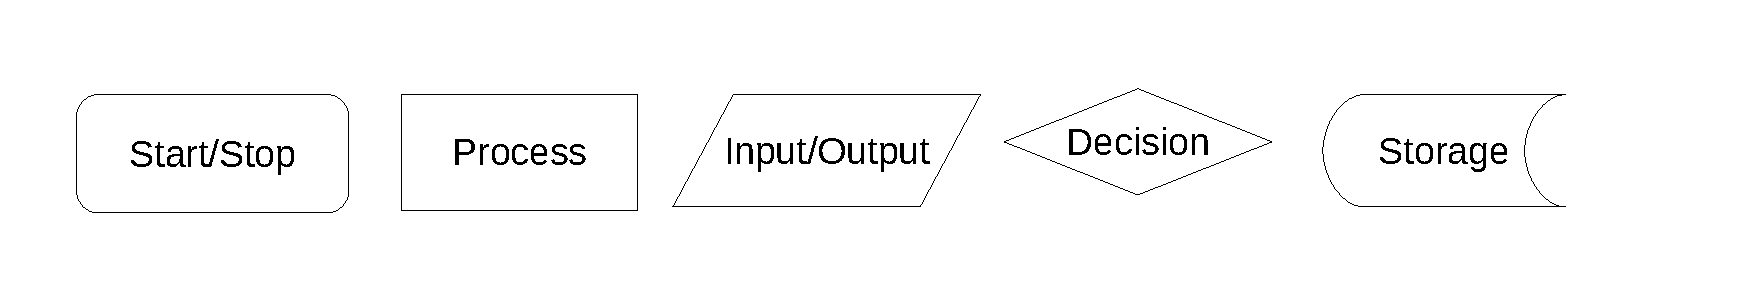
\includegraphics[width=\textwidth]{./Design/images/FC_key.pdf}
    \caption{Key for flow chart} \label{fig:Flow Chart Key}
\end{figure}

Start of the flow chart:
\begin{figure}[H]
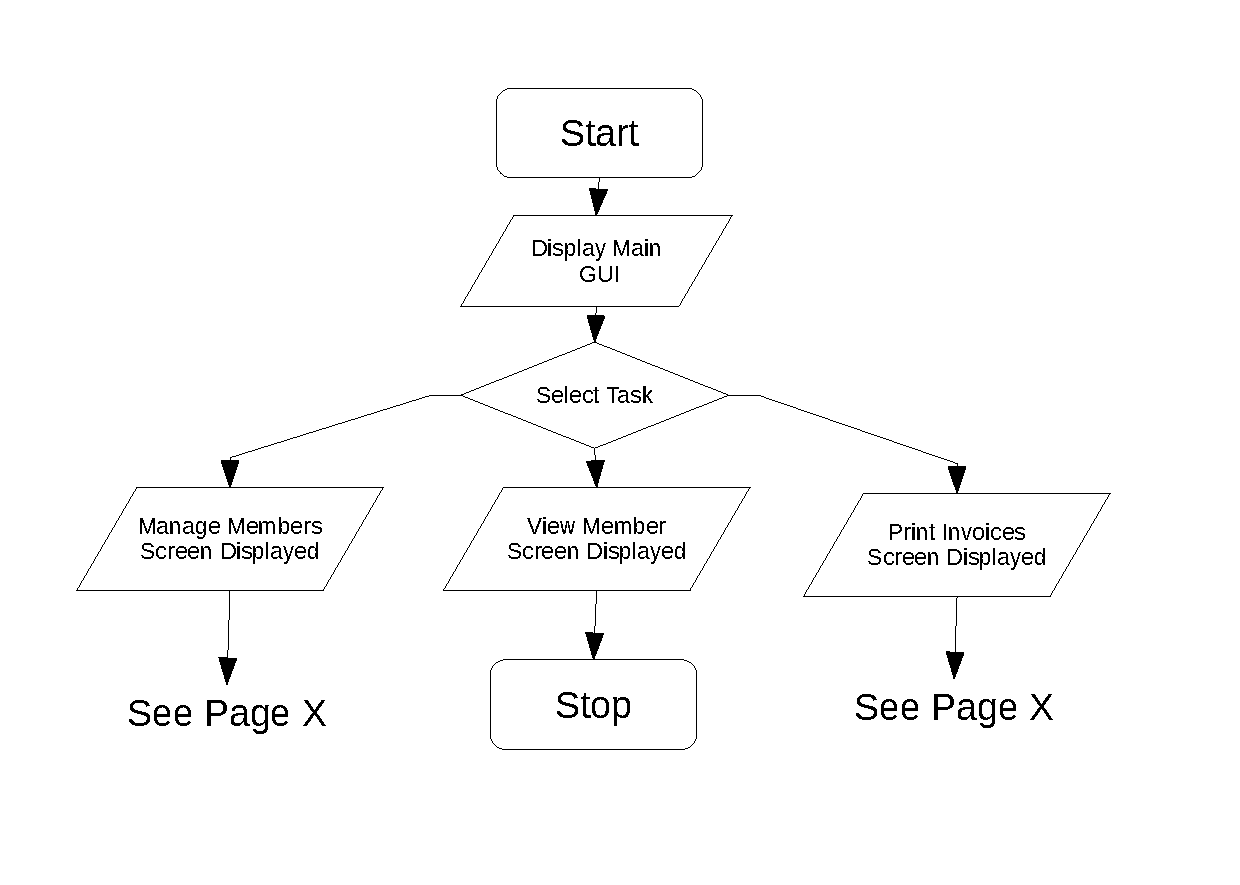
\includegraphics[width=\textwidth]{./Design/images/FC_start.pdf}
    \caption{Start of flow chart} \label{fig:Flow Chart Start}
\end{figure}

Managing members:
\begin{figure}[H]
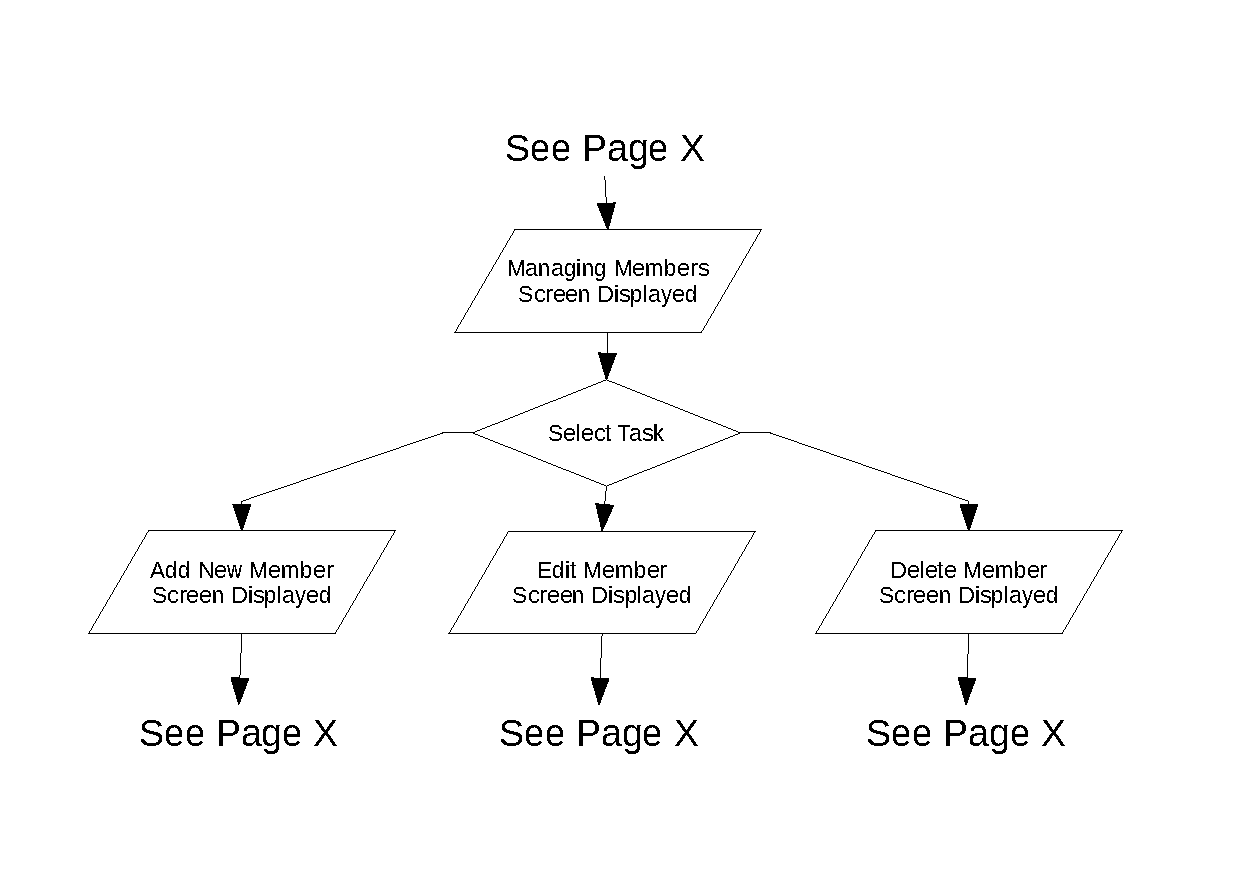
\includegraphics[width=\textwidth]{./Design/images/FC_manage_members.pdf}
    \caption{Manage Members} \label{fig:Flow Chart Manage Members}
\end{figure}

Editing a member:
\begin{figure}[H]
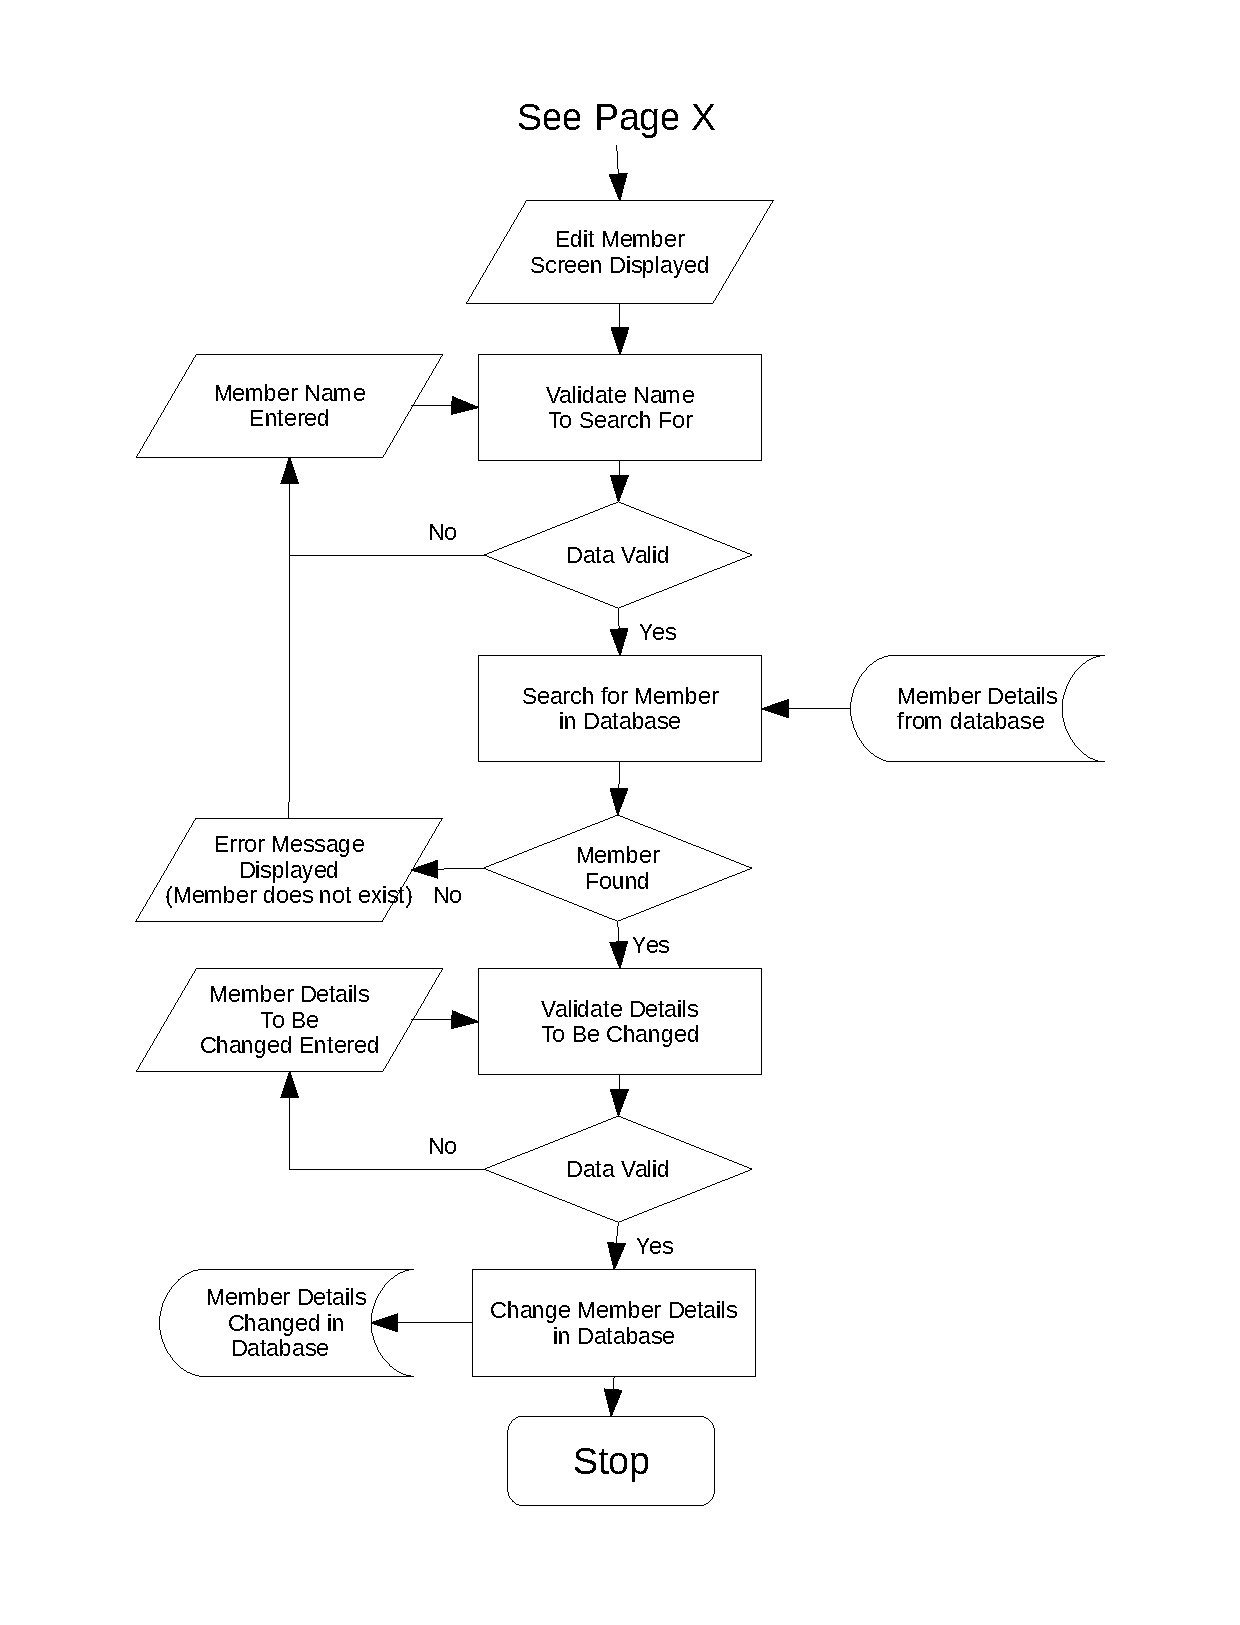
\includegraphics[width=\textwidth]{./Design/images/FC_edit_member.pdf}
    \caption{Edit Member} \label{fig:Flow Chart Edit Member}
\end{figure}

Deleting a member:
\begin{figure}[H]
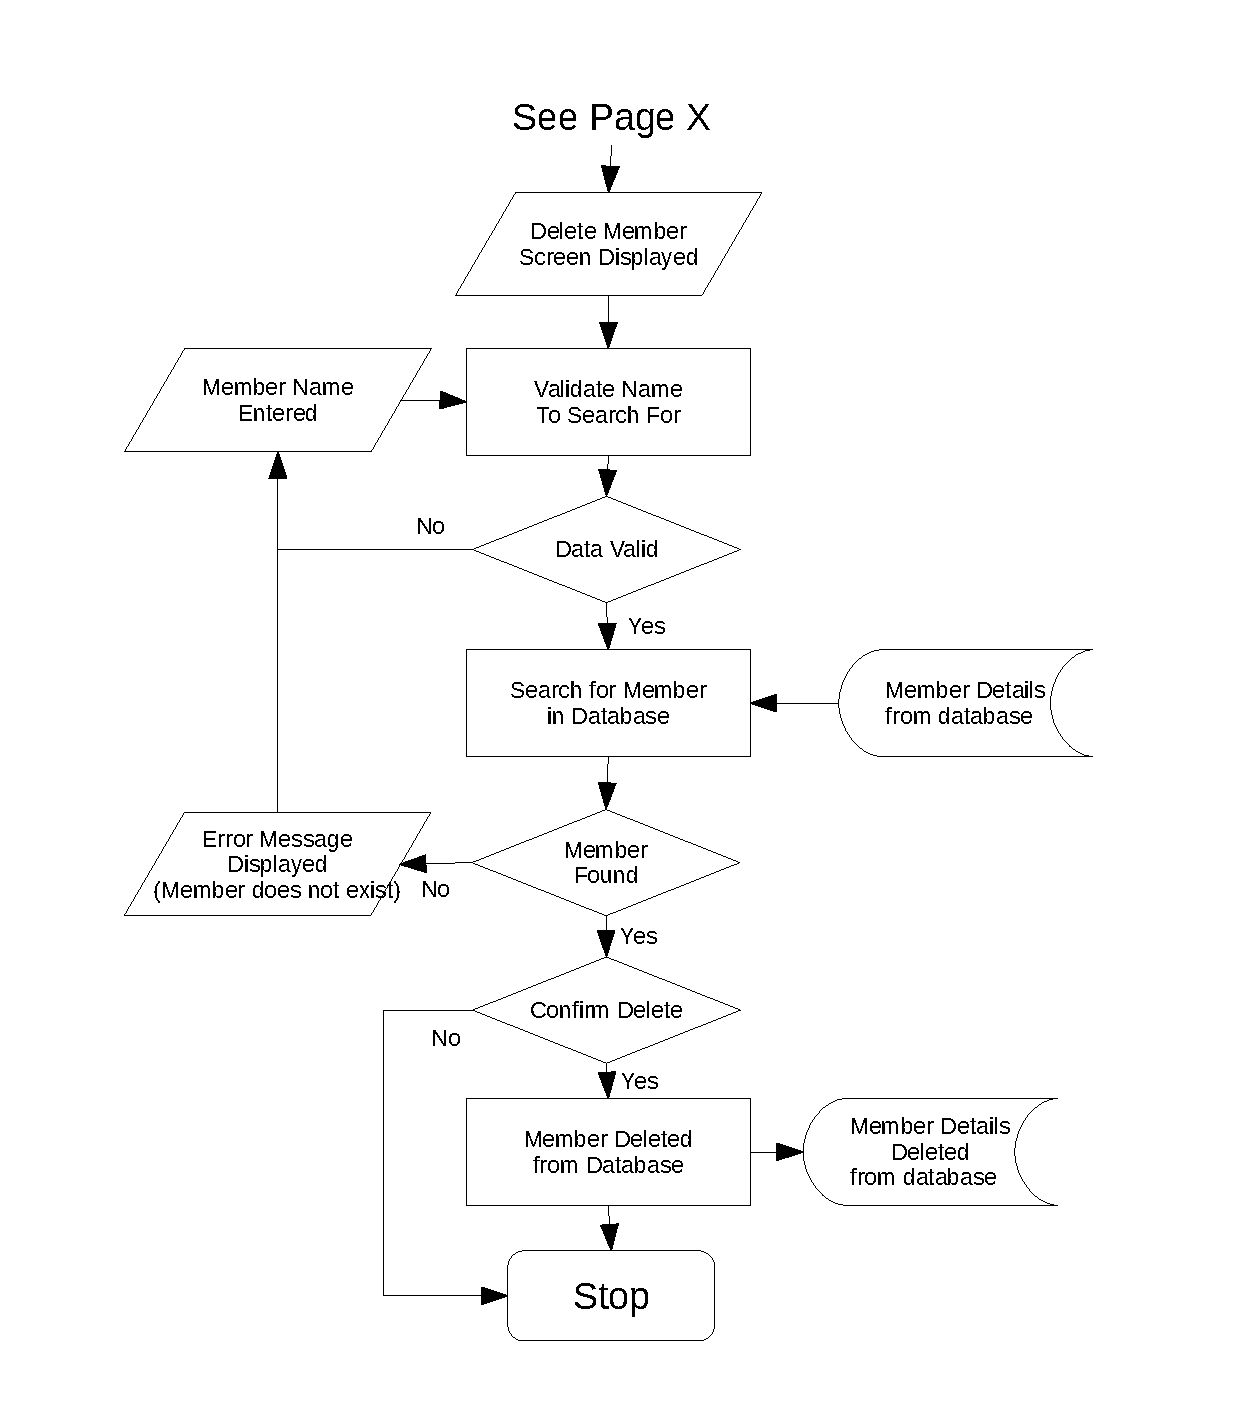
\includegraphics[width=\textwidth]{./Design/images/FC_delete_member.pdf}
    \caption{Delete Member} \label{fig:Flow Chart Delete Member}
\end{figure}

Adding a new member:
\begin{figure}[H]
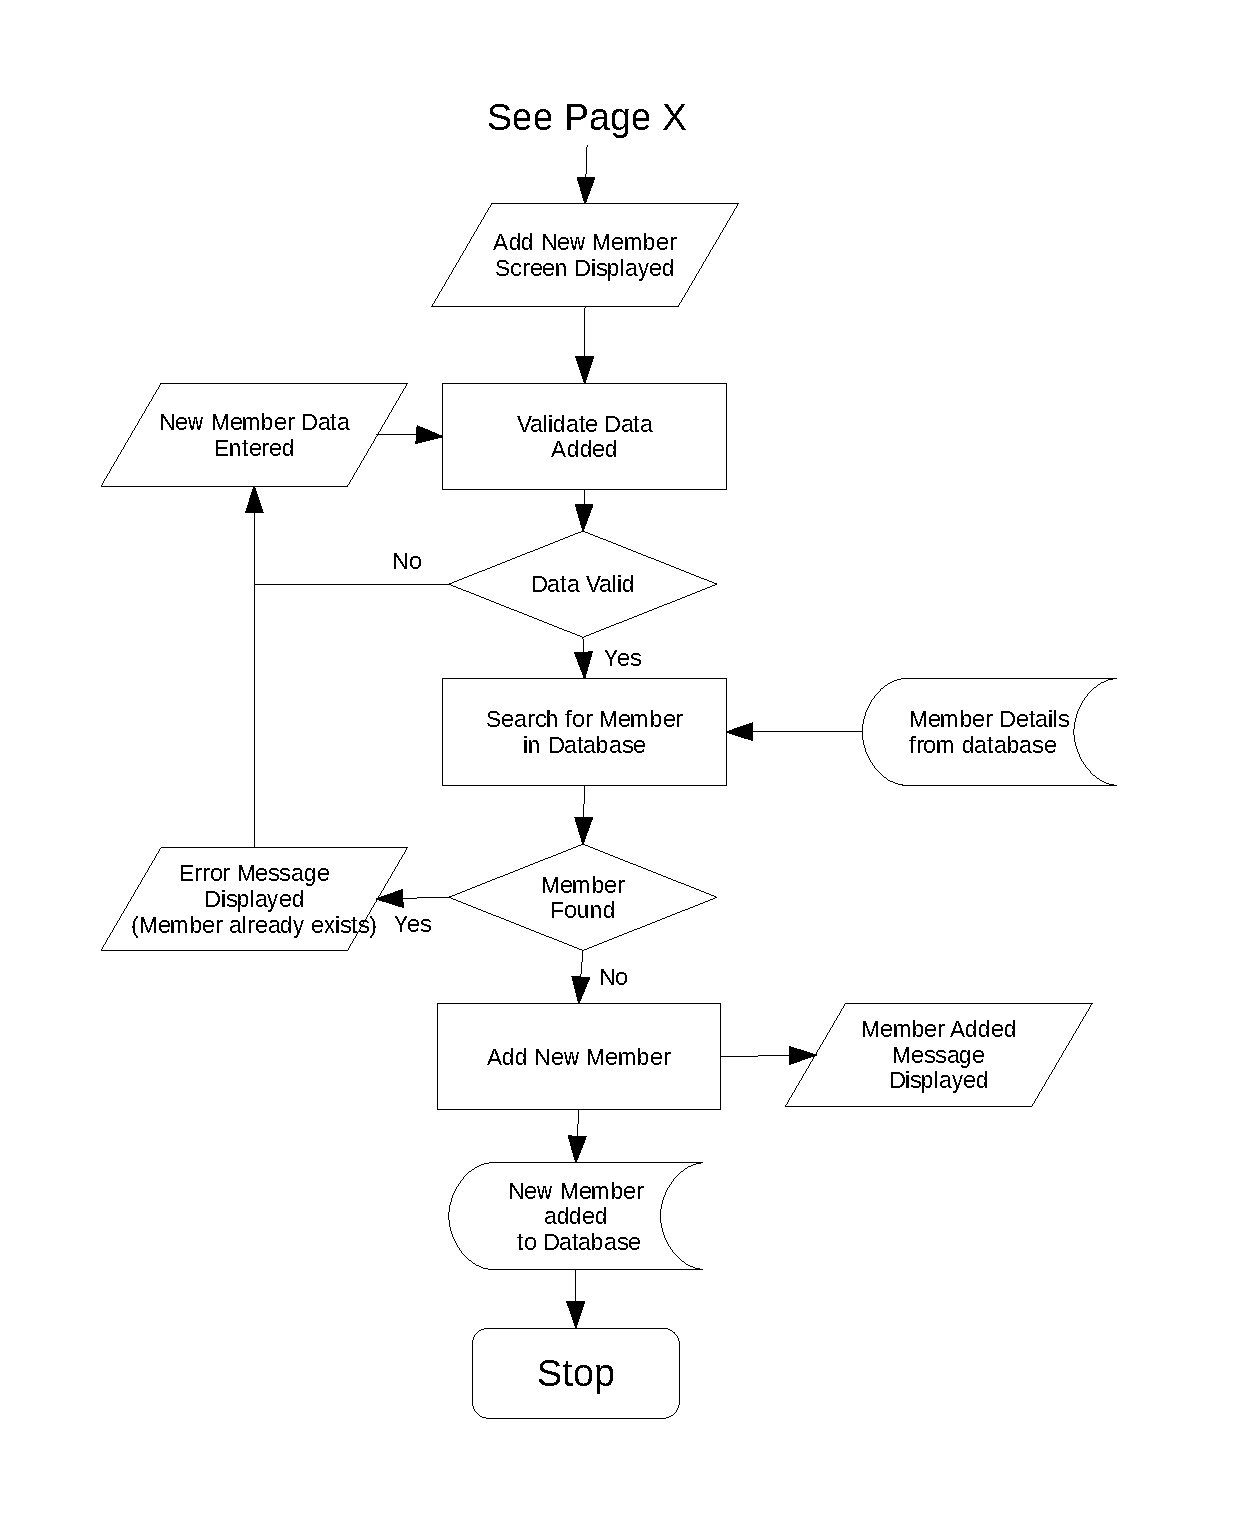
\includegraphics[width=\textwidth]{./Design/images/FC_add_new_member.pdf}
    \caption{Add New Member} \label{fig:Flow Chart Add New Member}
\end{figure}

Printing the invoices:
\begin{figure}[H]
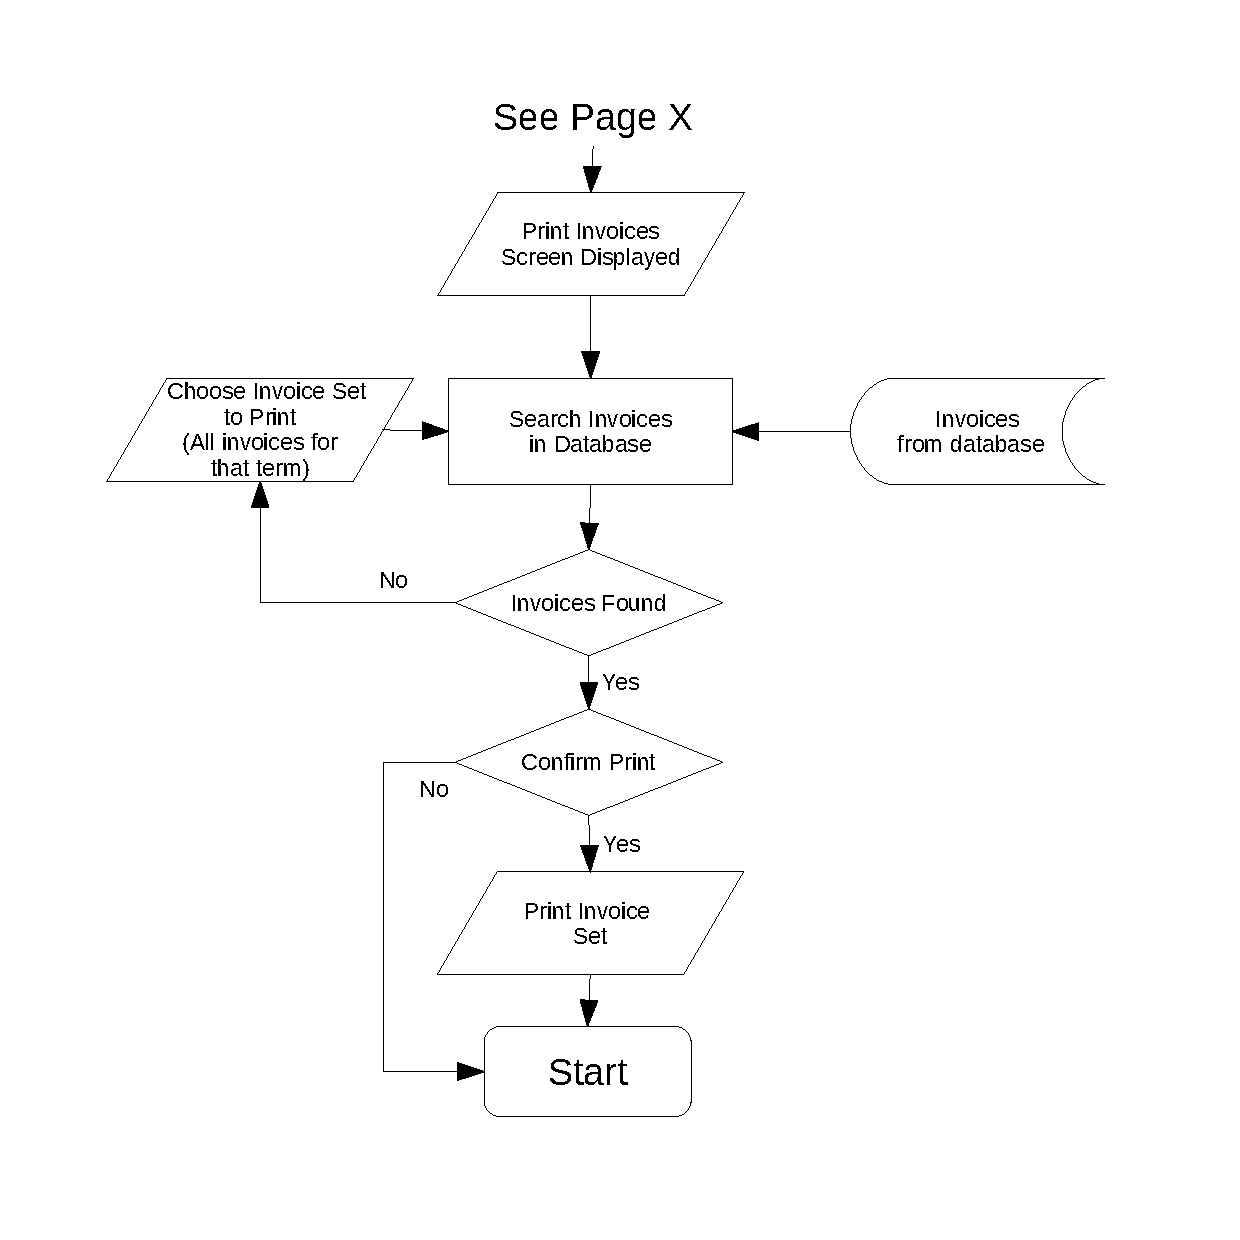
\includegraphics[width=\textwidth]{./Design/images/FC_print_invoices.pdf}
    \caption{Print Invoices} \label{fig:Flow Chart Print Invoices}
\end{figure}

\section{User Interface Designs}

Main window (Displays the database):
\begin{figure}[H]
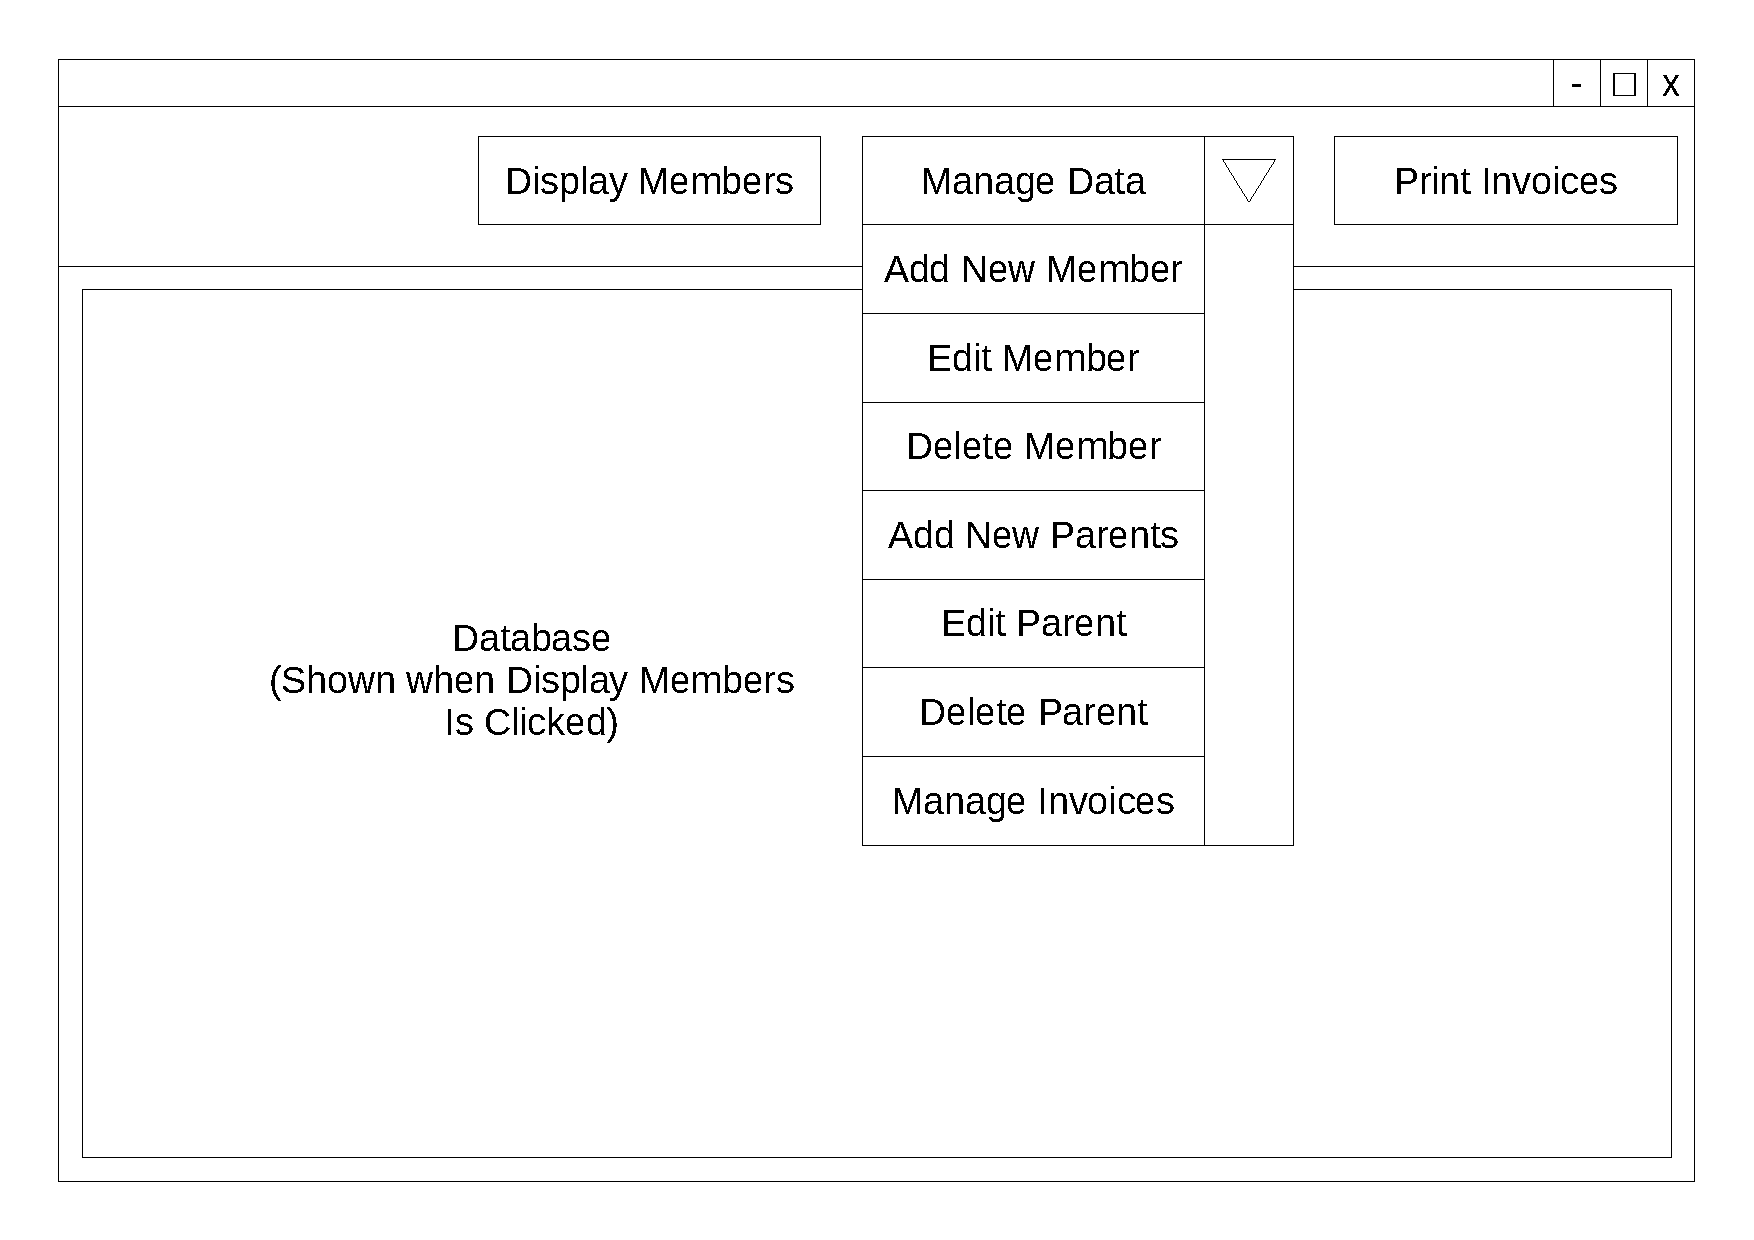
\includegraphics[width=\textwidth]{./Design/images/Main_Interface_Design.pdf}
    \caption{Main Interface} \label{fig:Interface Design}
\end{figure}
This is the main window. It will have a large area for displaying the database when the ``Display Members'' button is clicked and a dropdown menu to select functions to manipulate the data, and a button for printing invoices.

Most of the window will be taken up by the database as this is the main purpose of the program, and a larger box means that many fields can be compared by the user at once. The menu bar is at the top so as not to break up the viewing of the database. Most features will come under managing data so the menu bar is not too cluttered and the program can be easily navigated.

Adding a new member:
\begin{figure}[H]
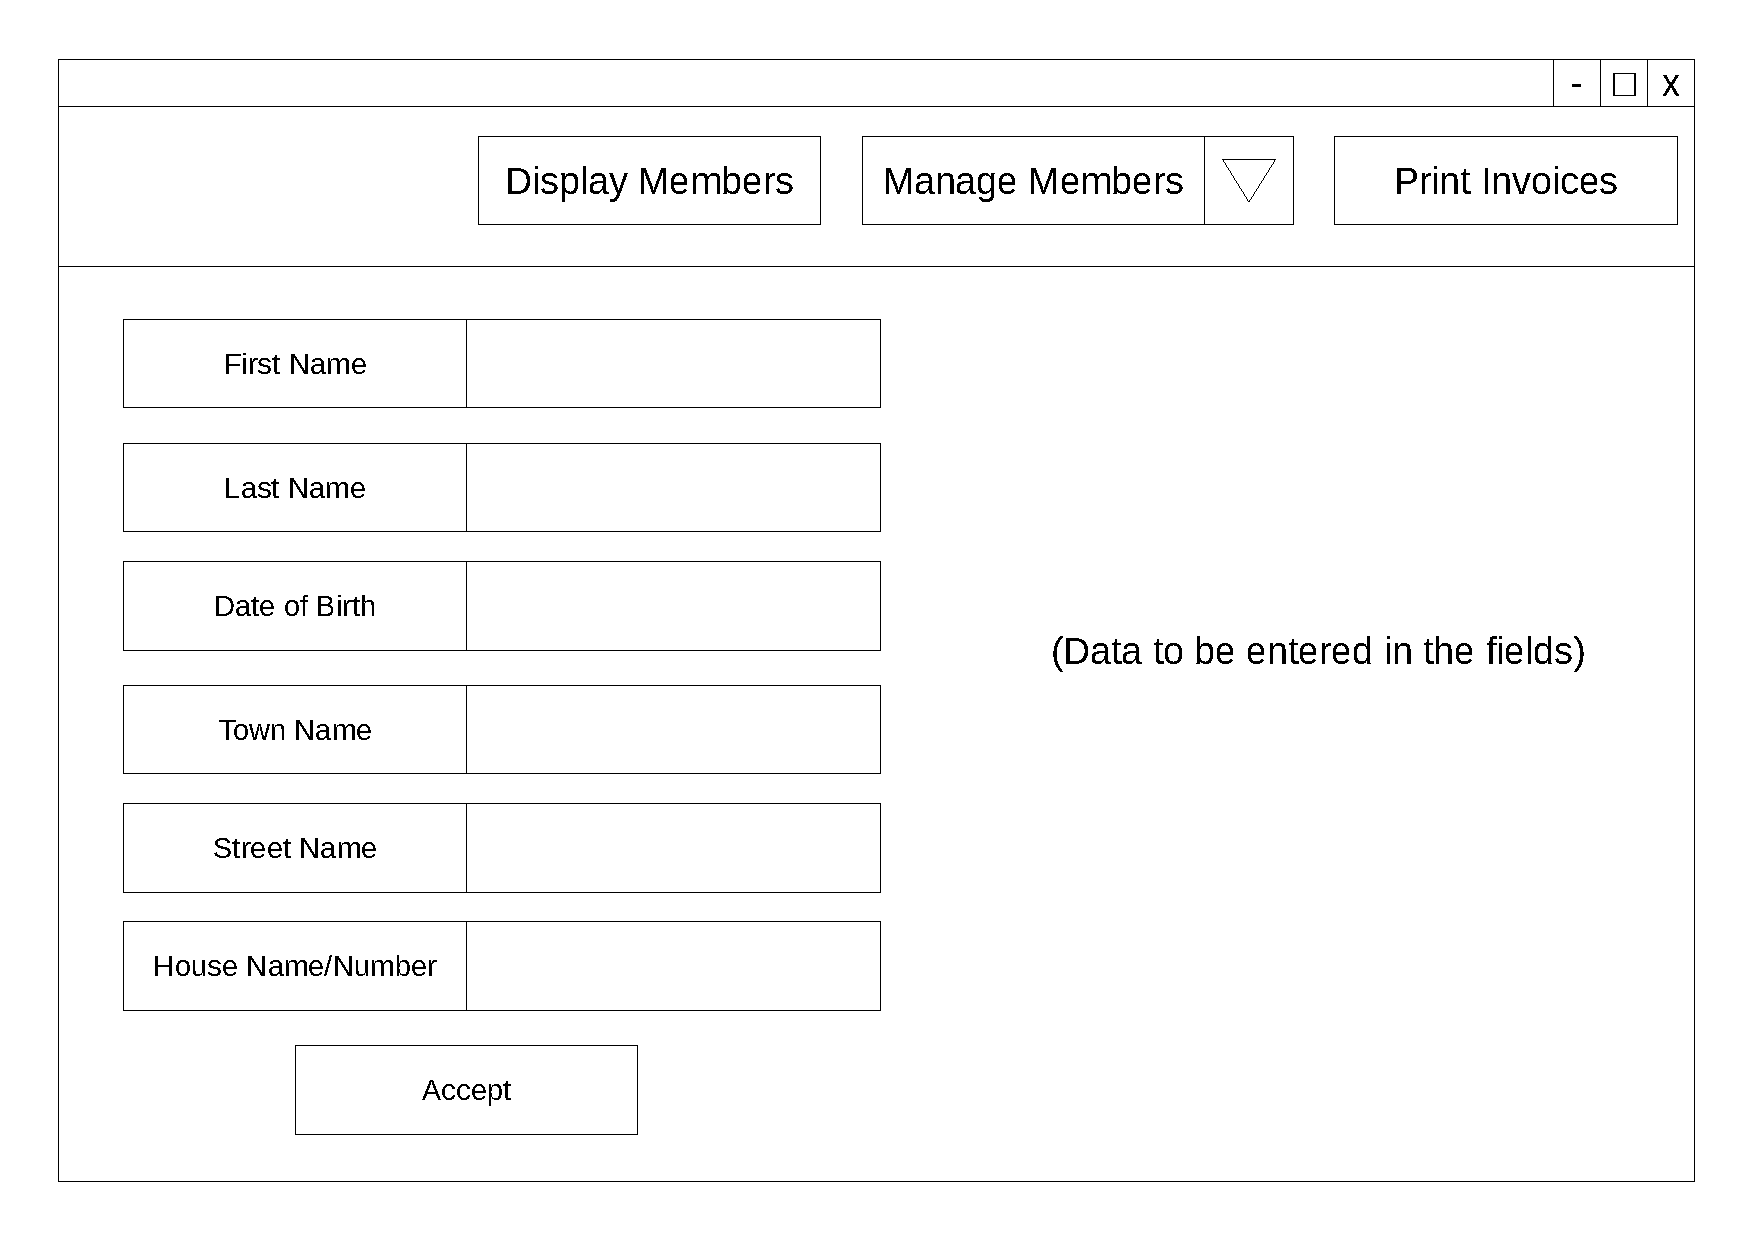
\includegraphics[width=\textwidth]{./Design/images/Add_New_Member.pdf}
    \caption{Add New Member} \label{fig:Interface Design}
\end{figure}
The area showing the database will be replaced with a new window with multiple fields to fill in. The data will not be accepted until all the fields are filled in with valid data, and the accept button is pressed.

The fields are labeled so the user can easily understand what data to input into them. The accept button is at the bottom so, assuming the user enters data from the top down, the flow will not be disrupted. The screen will persist with the data alreadt in the fields so siblings can be easily added.

Edit member screen 1 (Finding the member to be changed):
\begin{figure}[H]
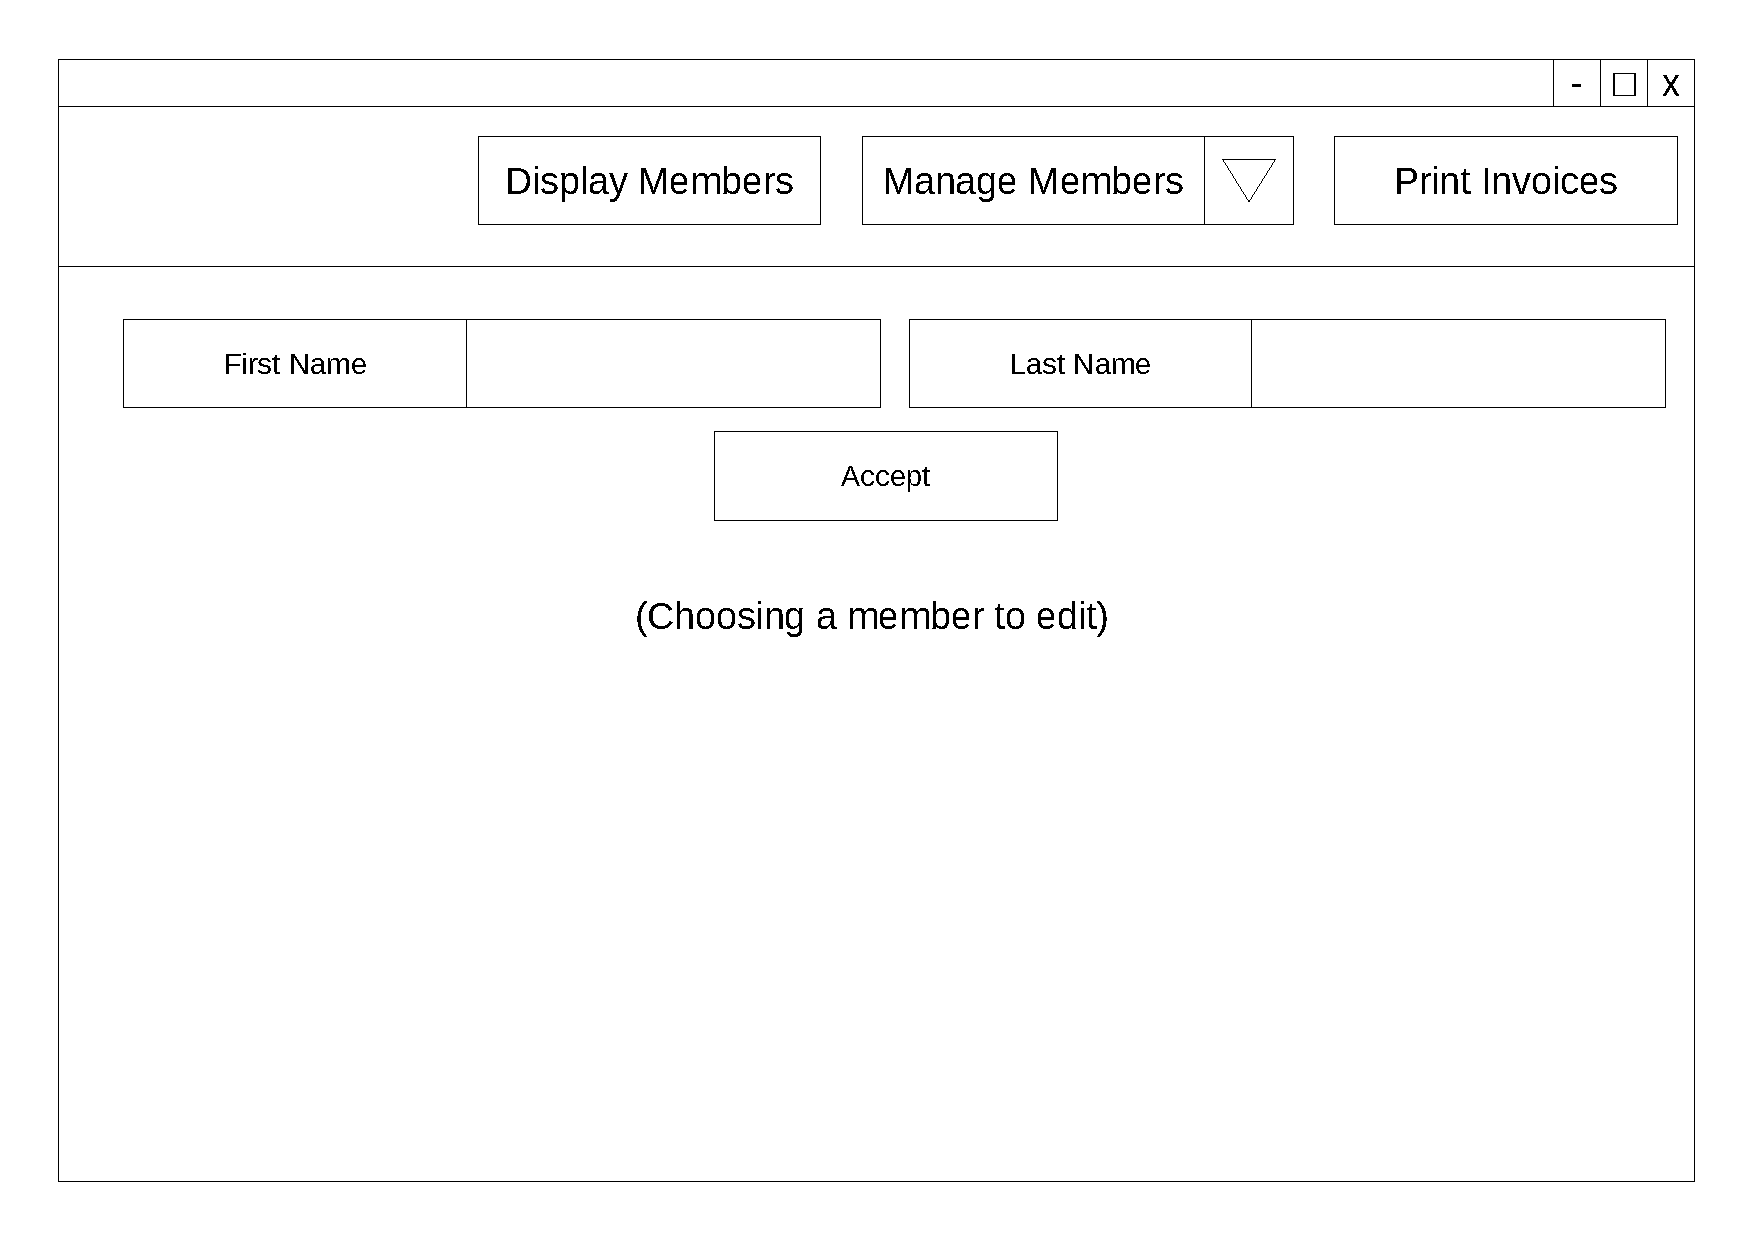
\includegraphics[width=\textwidth]{./Design/images/Edit_Member_1.pdf}
    \caption{Edit Member} \label{fig:Interface Design}
\end{figure}
The area showing the database will be replaced with a new window with two fields. The purpose of this window is to find the member to be edited. The second editing member screen will then show.

The first name and last name fields are used as these will almost certainly be unique to one individual, and should be easily memorable for the leaders, unlike things like addresses or data of births.

Edit member screen 2 (Adding new data):
\begin{figure}[H]
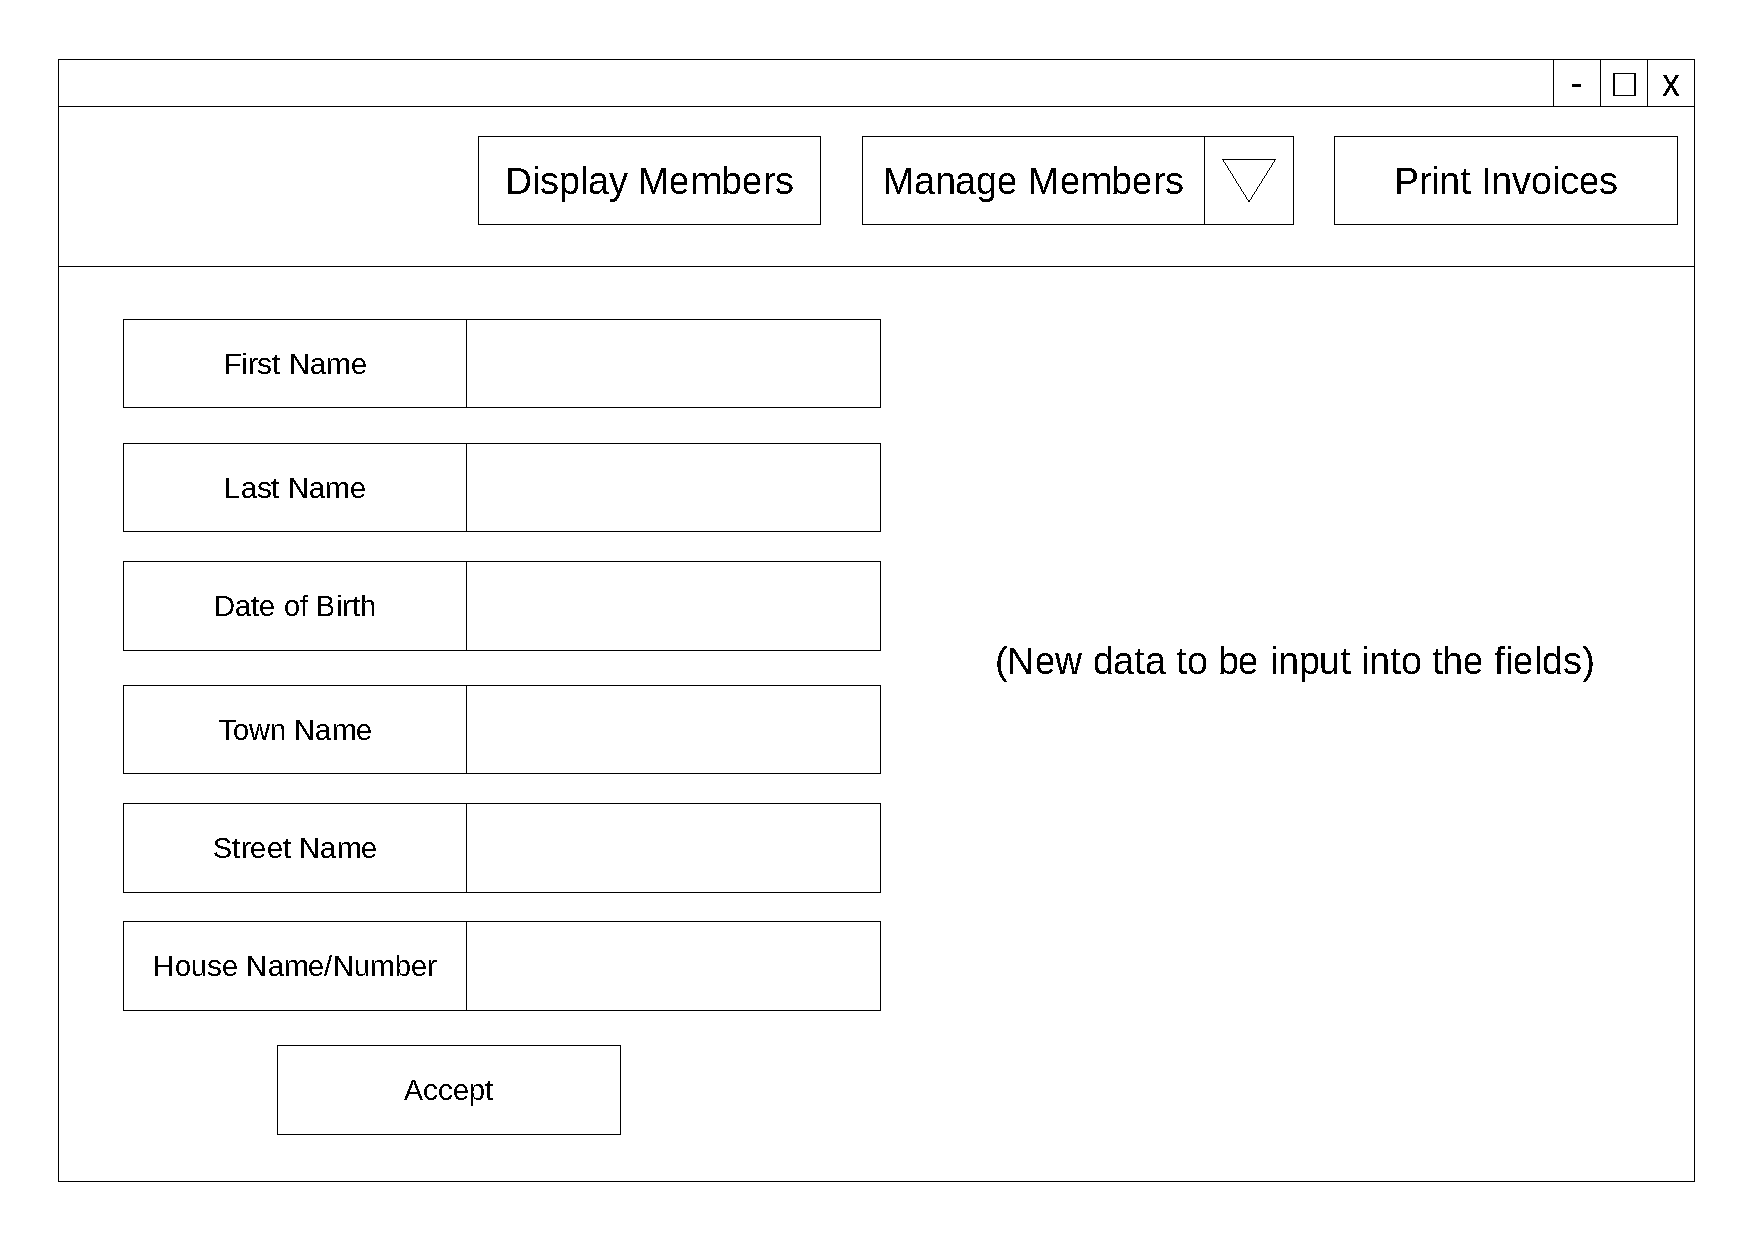
\includegraphics[width=\textwidth]{./Design/images/Edit_Member_2.pdf}
    \caption{Edit Member} \label{fig:Interface Design}
\end{figure}
This screen will only show when the member is found. Any data entered will be changed in the database. If a field is left blank then the data will not be changed.

Multiple fields can be edited at once so the accept button does not have to be clicked for each piece of new data. The accept button is underneath the fields to continue the flow.

Adding a new parent or a new invoice and editing a parent will be very similar to adding a new member and editing a member.



\section{Hardware Specification}
The system will need a desktop or computer running a Windows OS. A keyboard and a mouse will be needed to add information and to click buttons. Data will be stored on the internal hard drive of the computer and a monitor or display will be needed to show the GUI.

\section{Program Structure}

\subsection{Top-down design structure charts}

\begin{figure}[H]
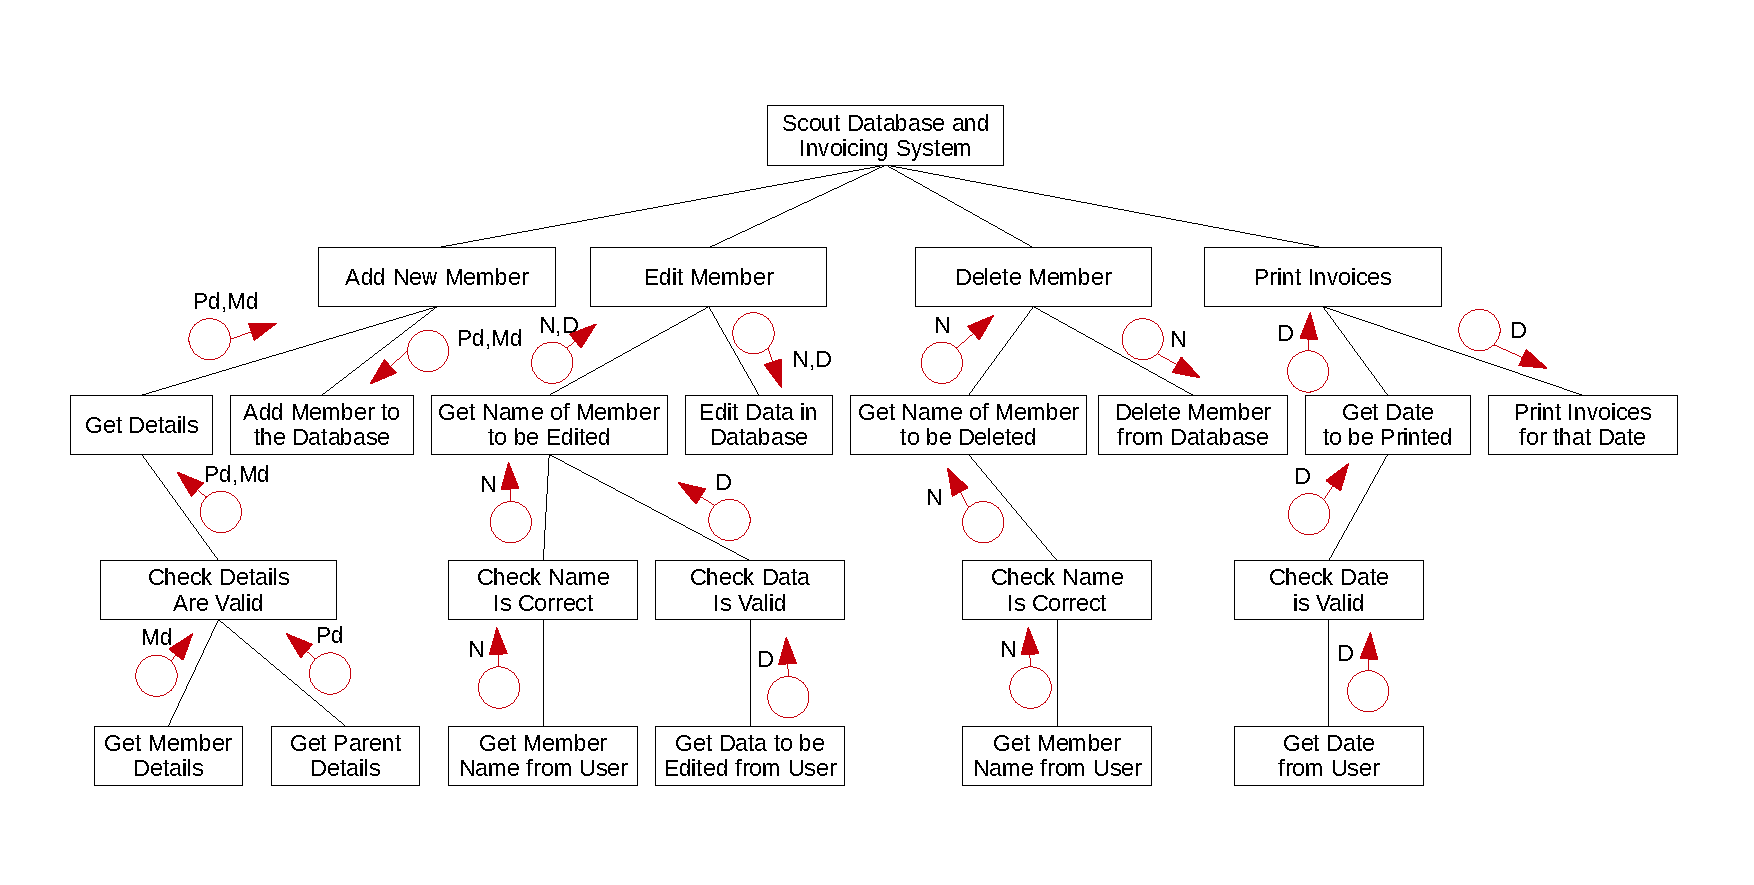
\includegraphics[width=\textwidth]{./Design/images/Design_Structure_Chart.pdf}
    \caption{Design Structure Chart} \label{fig:Structure_Chart}
\end{figure}

\subsection{Algorithms in pseudo-code for each data transformation process}

\begin{algorithm}[H]
\label{fig:check_username_and_password}
    \caption{FUNCTION CheckPassword(Password):}
\begin{algorithmic}[1]
\SEND{$"Please\ enter\ your\ password:\ "$}
\RECEIVE{$user\_password$}
\If{$user\_password = password$}
\SEND{$"Password \ is \ valid"$}
\SET{$password\_valid$}{$True$}
\Else
\SEND{$"Password \ not \ valid"$}
\SET{$password\_valid$}{$False$}
\EndIf
\end{algorithmic}
\end{algorithm}

\subsection{Object Diagrams}

\begin{figure}[H]
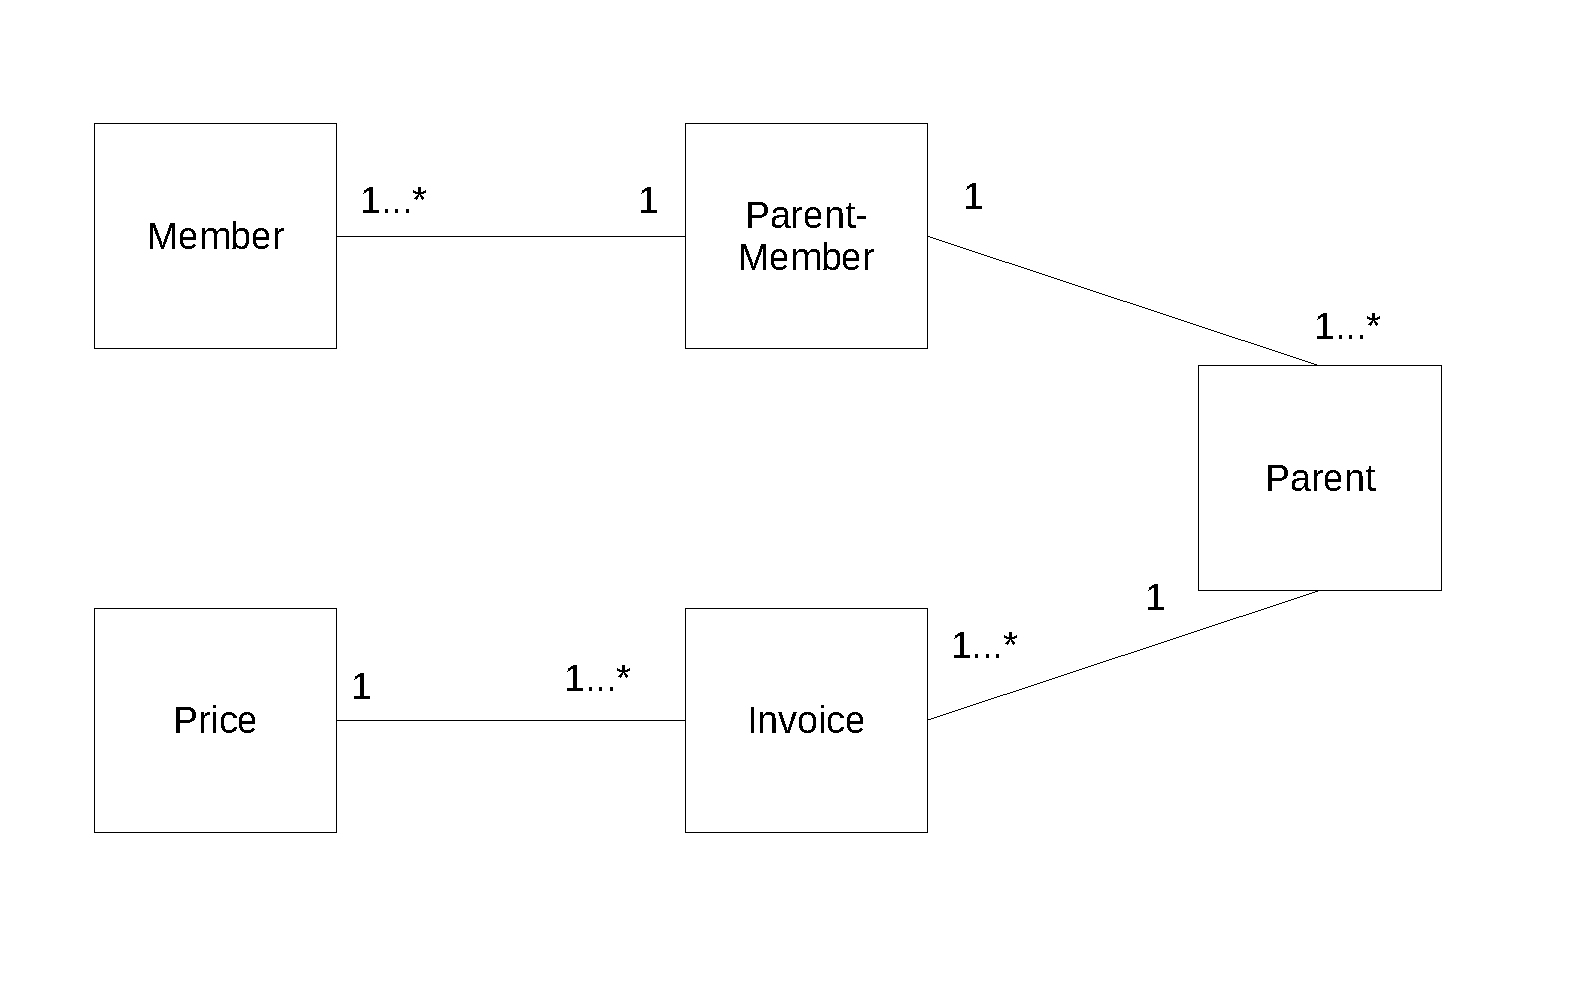
\includegraphics[width=\textwidth]{./Design/images/Relationship_Diagram.pdf}
    \caption{Relationship Diagram} \label{fig:Relationship Diagram}
\end{figure}

\subsection{Class Definitions}

Class Definitions:
\begin{figure}[H]
\includegraphics[width=\textwidth]{./Design/images/Class_definitions.pdf}
    \caption{Class Definitions} \label{fig:Interface Design}
\end{figure}

\section{Prototyping}
I will prototype a system that uses a python program to create a word document, save it to the harddrive in a pretermined location and print the document automatically.

In the real program, when the print invoices button is pressed a window will pop up asking the user which date they would like to print invoices from. When chosen, a new invoice document will be created for each parent and will be printed.

\section{Definition of Data Requirements}

\subsection{Identification of all data input items}

\begin{itemize}
	\item Member First Name
	\item Member Last Name
	\item Member Town Name
	\item Member Street Name
	\item Member House Name/Number
	\item Member Date of Birth
	\item Parent First Name
	\item Parent Last Name
	\item Parent Town Name
	\item Parent Street Name
	\item Parent House Name/Number
	\item Parent Phone Number
	\item Parent Email
	\item Was Invoice Paid
	\item Date Invoice Was Sent
\end{itemize}

\subsection{Identification of all data output items}

\begin{itemize}
	\item Price of member per term
\end{itemize}
Output to database:
\begin{itemize}
	\item Member First Name
	\item Member Last Name
	\item Member Town Name
	\item Member Street Name
	\item Member House Name/Number
	\item Member Date of Birth
	\item Parent First Name
	\item Parent Last Name
	\item Parent Town Name
	\item Parent Street Name
	\item Parent House Name/Number
	\item Parent Phone Number
	\item Parent Email
	\item Was Invoice Paid
	\item Date Invoice Was Sent
\end{itemize}

\subsection{Explanation of how data output items are generated}

\begin{center}
	\begin{tabular}{|p{6cm}|p{6cm}|l}
		\hline
		\textbf{Outpt}                   & \textbf{How the data is output} \\ \hline   
		Price of member per term   & Worked out from term price and number of siblings \\ \hline
		Member first name              & Taken from inputs            \\ \hline
		Member last name               & Taken from inputs          \\ \hline
		Member town name             & Taken from inputs        \\ \hline
		Member street name            & Taken from inputs       \\ \hline  
		Member house name/number & Taken from inputs          \\ \hline
		Member date of birth           & Taken from inputs          \\ \hline
		Parents first name               & Taken from inputs             \\ \hline
		Parent last name                 & Taken from inputs              \\ \hline
		Parent town name               & Taken from inputs          \\ \hline
		Parent street name             & Taken from inputs           \\ \hline
		Parent house name/number & Taken from inputs            \\ \hline 
		Parent phone number         & Taken from inputsr             \\ \hline
		Parent email                         & Taken from inputs                \\ \hline
		Was invoice paid                  & Taken from inputs             \\ \hline
		Date invoice was sent          & Taken from inputs             \\ \hline
	\end{tabular}
\end{center}

\subsection{Data Dictionary}

\newpage
\begin{center}
	\begin{tabular}{|p{2cm}|p{2cm}|p{2cm}|p{2cm}|l}
		\hline
		\textbf{Name}                    & \textbf{Data Type}    & \textbf{Length}                  & \textbf{Validation} \\ \hline
		MemberID                           & String            & 4 digits                & Numbers only \\ \hline
		ParentID                             & String            & 4 digits                & Numbers only \\ \hline
		Member first name              & String            & 1-20 characters   & Letters only \\ \hline
		Member last name               & String           &1-20 characters &  Letters only \\ \hline
		Parents first name               & String           & 1-20 characters &  Letters only \\ \hline
		Parent last name                 & String           & 1-20 characters &  Letters only \\ \hline
		Member town name                 & String           & 1-20 characters &  Letters only \\ \hline
		Member street name                 & String           & 1-20 characters &  Letters only \\ \hline
		Member house name/number & String              & 1-20 characters &  Letters only \\ \hline
		Parent town name                 & String           & 1-20 characters &  Letters only \\ \hline
		Parent street name                 & String           & 1-20 characters &  Letters only \\ \hline
		Parent house name/number & String                 & 1-20 characters &  Letters only \\ \hline
		Parent phone number         & Integer        & 12 digits & Numbers only, correct format and a valid phone number \\ \hline
		Parent email                        & String          & 1-30 characters &  Letters only \\ \hline
		Member date of birth          & Datetime       & 6 digits & Numbers only (dd/mm/yy) \\ \hline
		Invoice ID                           & Integer       & 4 digits & Numbers only \\ \hline
		Was invoice paid                 & Integer       & 4-6 digits & Numbers only, correct format and a valid date \\ \hline
		Date invoice was sent        & Datetime       & 6 digits & Numbers only (dd/mm/yy) \\ \hline
\end{tabular}
\end{center}

\subsection{Identification of appropriate storage media}

\section{Database Design}

\subsection{Normalisation}

\subsubsection{ER Diagrams}

ER diagram of the fully normalised database:
\begin{figure}[H]
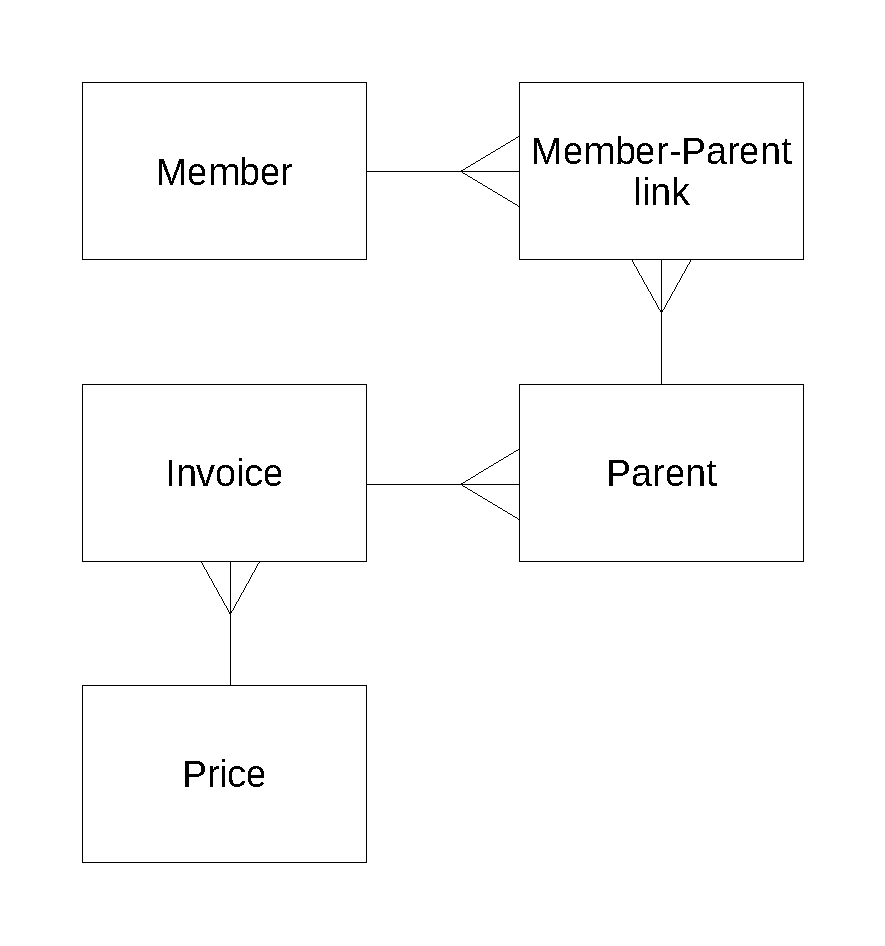
\includegraphics[width=\textwidth]{./Design/images/ER_diagram_design.pdf}
    \caption{ER diagram of the fully normalised database} \label{fig:ER_diagram_design}
\end{figure}


\subsubsection{Entity Descriptions}

\subsubsection{1NF to 3NF}

\textbf{\textit{UNF}}
\begin{center}
	\begin{tabular}{|p{4cm}|p{4cm}|}
		\hline
		MemberID \\ \hline
		ParentID \\ \hline
		Member First Name  \\ \hline
		Member Last Name \\ \hline
		Parent First Name \\ \hline
		Parent Last Name \\ \hline
		Member Town Name \\ \hline
		Member Street Name \\ \hline
		Member House Name/Number \\ \hline
		Parent Town Name \\ \hline
		Parent Street Name \\ \hline
		Parent House Name/Number \\ \hline
		Member Date of Birth \\ \hline
		Primary Parent Phone Number \\ \hline
		Secondary Parent Phone Number \\ \hline
		Parent Email \\ \hline
		InvoiceID \\ \hline
		Was invoice paid \\ \hline
		Date invoice was sent \\ \hline
		PriceID \\ \hline
		Term Price \\ \hline
		Sibling discount amount \\ \hline
	\end{tabular}
\end{center}

1. Split the attributes into repeating and non-repeating groups. Create a composite key in the repeating group.

\textbf{\textit{1NF}}
\textbf{\textit{Repeating}}
\begin{center}
	\begin{tabular}{|p{4cm}|p{4cm}|}
		\hline
		\textbf{ParentID} \\ \hline
		\textit{MemberID} \\ \hline
		Parent First Name \\ \hline
		Parent Last Name \\ \hline
		Parent Town Name \\ \hline
		Parent Street Name \\ \hline
		Parent House Name/Number \\ \hline
		Parent Phone Number \\ \hline
		Parent Email \\ \hline
		InvoiceID \\ \hline
		Was invoice paid \\ \hline
		Date invoice was sent \\ \hline
	\end{tabular}
\end{center}

\textbf{\textit{Non-Repeating}}
\begin{center}
	\begin{tabular}{|p{4cm}|p{4cm}|}
		\hline
		\textbf{MemberID} \\ \hline
		Member First Name  \\ \hline
		Member Last Name \\ \hline
		Member Town Name \\ \hline
		Member Street Name \\ \hline
		Member House Name/Number \\ \hline
		Member Date of Birth \\ \hline		
		PriceID \\ \hline
		Term Price \\ \hline
		Sibling discount amount \\ \hline
	\end{tabular}
\end{center}

2. Remove any attributes that do not rely on both parts of the composite key from the repeating group and add the key they do rely on to the new group.

\textbf{\textit{2NF}}
\begin{center}
	\begin{tabular}{|p{4cm}|p{4cm}|}
		\hline
		\textbf{MemberID} \\ \hline
		Member First Name  \\ \hline
		Member Last Name \\ \hline
		Member Town Name \\ \hline
		Member Street Name \\ \hline
		Member House Name/Number \\ \hline
		Member Date of Birth \\ \hline		
		PriceID \\ \hline
		Term Price \\ \hline
		Sibling discount amount \\ \hline
	\end{tabular}
\end{center}

\textbf{\textit{(a)}}
\begin{center}
	\begin{tabular}{|p{4cm}|p{4cm}|}
		\hline	
		\textbf{ParentID} \\ \hline
		\textit{MemberID} \\ \hline
	\end{tabular}
\end{center}

\textbf{\textit{(b)}}
\begin{center}
	\begin{tabular}{|p{4cm}|p{4cm}|}
		\hline
		\textbf{ParentID} \\ \hline
		\textit{MemberID} \\ \hline
		Parent First Name \\ \hline
		Parent Last Name \\ \hline
		Parent Town Name \\ \hline
		Parent Street Name \\ \hline
		Parent House Name/Number \\ \hline
		Parent Phone Number \\ \hline
		Parent Email \\ \hline
		InvoiceID \\ \hline
		Was invoice paid \\ \hline
		Date invoice was sent \\ \hline
	\end{tabular}
\end{center}

3. Split the new group further so all attributes are in a group with a primary key they directly relate to.

\textbf{\textit{3NF}}
\begin{center}
	\begin{tabular}{|p{4cm}|p{4cm}|}
		\hline
		\textbf{MemberID} \\ \hline
		Member First Name  \\ \hline
		Member Last Name \\ \hline
		Member Town Name \\ \hline
		Member Street Name \\ \hline
		Member House Name/Number \\ \hline
		Member Date of Birth \\ \hline		
	\end{tabular}
\end{center}

\begin{center}
	\begin{tabular}{|p{4cm}|p{4cm}|}
		\hline
		\textbf{ParentID} \\ \hline
		Parent First Name \\ \hline
		Parent Last Name \\ \hline
		Parent Town Name \\ \hline
		Parent Street Name \\ \hline
		Parent House Name/Number \\ \hline
		Parent Phone Number \\ \hline
		Parent Email \\ \hline	
	\end{tabular}
\end{center}

\begin{center}
	\begin{tabular}{|p{4cm}|p{4cm}|}
		\hline
		\textbf{ParentID} \\ \hline
		\textit{MemberID} \\ \hline		
	\end{tabular}
\end{center}

\begin{center}
	\begin{tabular}{|p{4cm}|p{4cm}|}
		\hline
		\textbf{PriceID} \\ \hline
		Term Price \\ \hline
		Sibling discount amount \\ \hline		
	\end{tabular}
\end{center}

\begin{center}
	\begin{tabular}{|p{4cm}|p{4cm}|}
		\hline
		\textbf{InvoiceID} \\ \hline
		Was invoice paid \\ \hline
		Date invoice was sent \\ \hline		
	\end{tabular}
\end{center}

Member\textbf{(MemberID},Member First Name, Member Last Name, Member Town Name, Member Street Name, Member house Name/Number, Member Date of Birth)

Parent-Member({\textbf{ParentID},\textit{MemberID})

Parent(\textbf{ParentID}, Parent First Name, Parent Last Name, Parent Town Name, Parent Street Name, Parent house Name/Number,  Parent Email, Parent Phone Number)

Invoice(\textbf{InvoiceID}, \textit{ParentID}, \textit{PriceID}, Was Invoice Paid, Date Invoice Was Sent)

Price(\textbf{PriceID}, Term Price, Sibling Discount)

\subsubsection{SQL Queries}

Displaying a list of members in age order: \\
SELECT *  \\
FROM Member \\
ORDER BY MemberDateOfBirth \\

Displaying the whole database: \\
Select * \\
FROM Member, Parent, Invoice \\

\section{Security and Integrity of the System and Data}

\subsection{Security and Integrity of Data}
As the system will be storing data of minors, such as date of birth, name, and address, security must be strict as the data falls under the data protection act. There will only be one login and data should be kept as up to date as possible and should be encrypted until the correct user name and password is entered, or else the files containing the data could be viewed manually without proper authorisation. Validation will be used to ensure all data entered is feasible.

\subsection{System Security}
Access will be limited to one user name and password, which will be given to Terry when the system is set up.

\section{Validation}
My program will validate all locations where ambiguous data could be entered. This includes where names could be entered (1 to 20 letters), for dates (in the format DD/MM/YY) and for phone numbers (12 digits) and email (1 to 30 characters broken up by a @ in the middle). If erroneous data is entered the user will be warned if trying to accept however the validation can be overwritten in the rare cases the validation could be inncorrect (for example if a person's last name is very long).

\begin{center}
	\begin{tabular}{|p{2cm}|p{2cm}|p{2cm}|p{2cm}|l}
		\hline
		\textbf{Test Series}   & \textbf{Purpose of Test Series}   & \textbf{Testing Strategy}   & \textbf{Strategy Rationale} \\ \hline
		1                       & Validate input into member or parent first name  & John, 16, John Smith  & Numbers only \\ \hline
		ParentID                             & String            & 4 digits                & Numbers only \\ \hline
\end{tabular}
\end{center}

\section{Testing}

\begin{landscape}
\subsection{Outline Plan}

\begin{center}
	\begin{tabular}{|p{2cm}|p{2cm}|p{2cm}|p{2cm}|l}
		\hline
		\textbf{Test Series}   & \textbf{Purpose of Test Series}   & \textbf{Testing Strategy}   & \textbf{Strategy Rationale} \\ \hline
		1  & Validating names, numbers and other strings  & Bottom-up testing  & Components will be tested as they are developed \\ \hline
		2  & Check searching the database is working correctly & Bottom-up testing  & Components will be tested as they are developed \\ \hline
		3  & Check data is inserted into the database in the right locations & Bottom-up testing  & Components will be tested as they are developed \\ \hline
		4  & Check buttons and flow of control work as intented & Top-down testing  & Components will be tested when the program is finished to check buttons still retain their functionality \\ \hline
		5  & Test the GUI & Bottom-up testing  & Components will be tested as they are developed \\ \hline
\end{tabular}
\end{center}

\subsection{Detailed Plan}

\begin{center}
    \begin{longtable}{|p{1.5cm}|p{2.5cm}|p{2.5cm}|p{2cm}|p{2cm}|p{2cm}|p{2cm}|p{2cm}|}
        \hline
        \textbf{Test Series} & \textbf{Purpose of Test} & \textbf{Test Description} & \textbf{Test Data} & \textbf{Test Data Type (Normal/ Erroneous/ Boundary)} & \textbf{Expected Result} & \textbf{Actual Result} & \textbf{Evidence}\\ \hline
        1.1 & Validate first or last name is likely to be correct & Check the string consists of just letters and is between 1 and 20 characters and contains no spaces & John, 12345, John19, J, John Smith & Normal, Erroneous, Erroneous, Boundary, Erroneous & Accepted, Error, Error, Accepted, Error & \\ \hline
        1.2 & Validate town name is likely to be correct & Check the string consists of just letters, hyphens and spaces and is between 1 and 20 characters & Fordham, Walton-on-the-Naze, Bury St Edmunds, Soham19 & Normal, Normal, Normal, Erroneous & Accepted, Accepted, Accepted, Error & \\ \hline
        1.3 & Validate street name is likely to be correct & Check the string consists of just letters, hyphens and spaces and is between 1 and 20 characters & Market Street, Feast Close, ChurchStreet19 & Normal, Normal, Erroneous & Accepted, Accepted, Error & \\ \hline
        1.4 & Validate house name/number is likely to be correct & Check the string consists of just letters, hyphens and spaces and is between 1 and 20 characters OR is a number of 1 to 3 characters & Swan, 4, Swan4 & Normal, Normal, Erroneous & Accepted, Accepted, Error & \\ \hline
        1.5 & Validate phone number is likely to be correct & Check the string consists of just numbers and is 12 characters & 01234, 012345678911, one two three & Erroneous, Normal, Erroneous & Error, Accepted, Error & \\ \hline
        1.6 & Validate email is likely to be correct & Check the string consists of letters, ``@ `` and ``.`` 1 to  30 characters & johnsmith.co.uk, johnsmith@longroad.ac.uk, johnsmithatlongroad.ac.uk & Erroneous, Normal, Erroneous & Error, Accepted, Error & \\ \hline
        1.7 & Validate date of birth is likely to be correct & Check the string consists of just numbers and / and in the format DD/MM/YY & 15th November, 15/11/96, 15/11/1996, 15.11.96 & Erroneous, Normal, Erroneous, Erroneous & Error, Accepted, Error, Error & \\ \hline
        1.8 & Validate date the invoice was sent is likely to be correct & Check the string consists of just numbers and / and in the format DD/MM/YY & 1st January, 01/01/11, 01/01/2011, 01.01.11 & Erroneous, Normal, Erroneous, Erroneous & Error, Accepted, Error, Error & \\ \hline
        2.1 & Validate date of birth is likely to be correct & Check the string consists of just numbers and / and in the format DD/MM/YY & 15th November, 15/11/96, 15/11/1996, 15.11.96 & Erroneous, Normal, Erroneous, Erroneous & Error, Accepted, Error, Error & \\ \hline
    \end{longtable}
\end{center}
\end{landscape}
